\scanpage{12}
\uline{Remarques} 1.11. a) Le préschéma $\unsure{\mathcal T|\tau}$ de 6.10. s'appellera comme de juste le
\uline{préschéma des tores maximaux} de G. On verra au N°5 qu'il est en fait \uline{affine}
sur S. On peut le vérifier directement, lorsque G est isomorphe à un
sous-préschéma en groupes fermé d'un préschéma de la forme $\mathrm{Gl}(n)$, en
utilisant Exp XI 4.6. et en remarquant que par le raisonnement de la
démonstration de 1.7. b), $\unsure{\mathcal T|\tau}$ s'identifie à un sous-préschéma à la fois
\uline{ouvert et fermé} du préschéma F qui représente les sous-groupes de type
multiplicatif de G.

b) Il \deleted{ne serait pas difficile}\inserted{est possible} de donner une démonstration de 1.7.
donc de 1.9, n'utilisant pas les résultats délicats de Exp XI, mais
seulement \inserted{les \deleted{\unsure{anciens}} résultats faciles} Exp XI 3.12.
\deleted{\unsure{de Exp XI N°6}}\inserted{et 6.2.}
en travaillant uniquement avec des groupes
de type multiplicatif finis sur la base (moralement, les groupes $\,{}_nT$ où T
est un tore maximal), comparer \deleted{\unsure{au}} N°7.
\deleted{Par contre,}\inserted{La même remarque vaut pour} la démonstration
de 1.10.
\deleted{s'appuie de façon essentielle sur Exp XI 4.\unsure{1}.
Dans un autre
exposé, nous donnerons une version généralisée de 1.10. par une démonstration
différente (s'appuyant sur un théorème de représentabilité de EGA \unsure{V|VI}).
\deleted{Exception faite \unsure{du Exp N°5},}
\inserted{De façon générale,}\inserted{pour les résultats du N°5,}
les théorèmes de représentabilité de Exp XI
N°4 \deleted{\unsure{vraisemblablement}} pourraient\deleted{\unsure{tous}}
être éliminés de la théorie
présentée \inserted{dans le présent exposé et les suivants}.}
\deleted{\inserted{de façon générale,
il est possible (et sans doute avantageux) d'éliminer
totalement les résultats de représentabilité de
Exp $\overline{\underline{\mathrm{XI}}}$ N°4 de la théorie présentée dans le
présent exposé et les suivants.}}
\margin{\figure{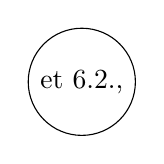
\begin{tikzpicture}[baseline=(t.base)]
\node[draw,circle,inner sep=3pt] (t) {et 6.2.,};\end{tikzpicture}}}
\margin{11}
